\documentclass[11pt,letterpaper]{article}
\usepackage[utf8]{inputenc}
\usepackage[T1]{fontenc}
\usepackage[spanish,es-nodecimaldot]{babel}
\usepackage[margin=2.1cm]{geometry}
\usepackage{booktabs,tabularx,xcolor,hyperref,enumitem,listings,fancyhdr,graphicx}
\hypersetup{colorlinks=true,linkcolor=blue,urlcolor=blue}
\pagestyle{fancy}\fancyhead{}\fancyfoot{}\fancyfoot[C]{\thepage}
\setlength{\parskip}{.4em}\setlength{\parindent}{0pt}
\lstset{basicstyle=\ttfamily\small,breaklines=true,frame=single,backgroundcolor=\color{gray!8}}

\title{\textbf{AlertaP}\\\large Detección temprana de sismos con deep learning}
\author{Javier Eduardo España Pacheco (23361)\\Angel Esteban Esquit Hernández (23221)\\
CC3092 Deep Learning y Sistemas Inteligentes\\Universidad del Valle de Guatemala}
\date{Noviembre de 2026}
\begin{document}
\maketitle
\begin{abstract}
AlertaP es un prototipo de alerta temprana sísmica que recibe ventanas de un
sismógrafo de tres componentes, detecta la llegada de la onda P y estima cuántos
segundos quedan antes de la onda S. Implementa un detector profundo de dos capas
ocultas, un baseline STA/LTA y un dashboard de demostración. La evaluación usa
60 ventanas reproducibles (30 eventos y 30 de ruido) y reporta error de picking,
precisión, recall, F1, latencia y valor económico neto. La decisión central del
proyecto es tratar el umbral como una decisión operativa: bajar el umbral puede
ganar anticipación, pero aumenta falsas alarmas y paros innecesarios.
\end{abstract}

\section{Problema, usuario y criterios de éxito}
Guatemala está en una zona de alta actividad sísmica. Para una planta industrial,
una señal temprana puede permitir detener maquinaria, cerrar una válvula de gas o
avisar a las personas antes de la llegada de la onda S, que suele ser más
destructiva. El usuario objetivo es el operador de una instalación con sensores
sísmicos y acciones automáticas definidas; el producto le entrega una alerta,
probabilidad, instante estimado y anticipación.

La hipótesis de partida es que un umbral fijo sobre la energía (STA/LTA) se
degrada con ruido cultural, variación de estación y amplitud, y que un modelo
profundo, que aprende patrones temporales y combina las tres componentes,
compensa esa degradación. Esta hipótesis se contrasta con un baseline justo en la
sección de evaluación y, como se verá, \textbf{no se confirma} sobre los datos
sintéticos actuales. No se afirma que el prototipo sea un sistema certificado: su
objetivo académico es medir el intercambio entre calidad técnica y valor de
negocio.

\textbf{Criterios de éxito:} recall $\geq 0.80$ en ventanas con evento; precisión
$\geq 0.80$ en el punto de operación elegido; error absoluto medio de picking
$<0.30$ s; latencia local $<2$ s; y valor positivo bajo los costos explícitos.

\section{Datos y pipeline}
\subsection{Fuente y preparación}
La propuesta define STEAD (Stanford Earthquake Dataset), con más de un millón de
registros de tres componentes y llegadas P/S etiquetadas, como fuente principal.
También propone validar con estaciones de Guatemala mediante FDSN/IRIS cuando haya
disponibilidad. En esta entrega se implementa una capa sintética controlada para
que el repositorio y las métricas sean ejecutables sin descargar gigabytes ni
depender de red. Cada ventana dura 12 s a 100 Hz y contiene Z, N y E. Los eventos
tienen una llegada P entre 2 y 5 s, una llegada S entre 1 y 2.8 s después, ruido
gaussiano y ondas amortiguadas; las ventanas negativas contienen únicamente
ruido. La semilla por defecto es 23361.

Para una integración real, los registros STEAD/FDSN deben convertirse a la misma
forma $(T,3)$, normalizarse por ventana, conservar sus etiquetas P/S y separarse
por evento/estación para evitar fuga entre entrenamiento y prueba. La señal se
filtra con un pasa-banda Butterworth de 1--18 Hz.

\subsection{Arquitectura}
\begin{center}
\begin{tabular}{c}
\fbox{Ventana de señal Z/N/E}\\$\downarrow$\\
\fbox{Filtrado y normalización}\\$\downarrow$\\
\fbox{Energía, envolvente, media móvil y gradiente}\\$\downarrow$\\
\fbox{MLP: 32 neuronas ReLU $\rightarrow$ 16 ReLU $\rightarrow$ probabilidad P}\\$\downarrow$\\
\fbox{Umbral $\rightarrow$ primera muestra candidata $\rightarrow$ alerta y anticipación}\\$\downarrow$\\
\fbox{Dashboard / acción operativa}
\end{tabular}
\end{center}

El modelo recibe cuatro variables por instante agregadas sobre las tres
componentes. Se entrena con Adam, 160 iteraciones máximas, validación interna
15\%, early stopping y semilla fija. Es una aproximación reproducible y liviana
a PhaseNet/EQTransformer; la siguiente iteración sustituye el extractor por una
CNN 1-D o fine-tuning de un picker preentrenado con STEAD.

\section{Modelo, baseline y decisión de umbral}
El baseline es STA/LTA causal: compara la energía media de una ventana corta de
0.25 s contra una larga de 3 s, ambas calculadas solo con muestras pasadas, y
alerta cuando el cociente supera un umbral (2.0, elegido por valor en
validación). Igual que DeepPhase, ignora el primer segundo, afectado por
transitorios del filtro. El modelo evaluado es
DeepPhase, un MLP de dos capas ocultas que estima $P(P\mid x_t)$. La inferencia
selecciona la primera muestra cuyo valor supera el umbral de decisión, que se
elige por valor de negocio en un conjunto de validación (0.85; ver sección~\ref{sec:valor}).

El problema es de deep learning supervisado sobre series temporales: el modelo
debe producir una decisión numérica auditable. La experiencia de usuario comunica probabilidad,
latencia, detector clásico y segundos hasta S. Una probabilidad no se presenta
como certeza.

\section{Evaluación}
El conjunto contiene 60 ventanas: 30 con evento y 30 de ruido, generadas con
semillas y distribuciones documentadas. La división conceptual es por ventana;
para validar con STEAD se debe dividir por evento y estación. Se reportan:
\begin{itemize}[leftmargin=*]
\item \textbf{Error de picking:} $|t_{\mathrm{pred}}-t_P|$ en segundos.
\item \textbf{Precisión/recall/F1:} un acierto exige aviso útil: alerta no
  anterior a $t_P-0.5$ s y anterior a la llegada de S. Una alerta tardía o
  prematura cuenta como evento no detectado (FN).
\item \textbf{Latencia:} tiempo de inferencia del detector.
\item \textbf{Valor:} función de la sección~\ref{sec:valor}, con costos explícitos de
  falsas alarmas, eventos no detectados y operación.
\end{itemize}
La división es de tres conjuntos independientes: entrenamiento (semilla 23361),
validación de 120 ventanas (semilla 777), donde se elige el umbral por valor, y
prueba de 60 ventanas (semilla 2026), donde se reportan los resultados.
La evaluación se ejecuta con \texttt{.venv/bin/python src/evaluate.py} y guarda
\texttt{results/metrics.json}; así no se reportan números escritos a mano.

\begin{table}[h]
\centering
\caption{Métricas en el conjunto de prueba, cada sistema en el umbral elegido por valor en validación.}
\begin{tabular}{lcccccc}
\toprule
Sistema & Umbral & Precisión & Recall & F1 & Error P (s) & Valor neto\\
\midrule
STA/LTA & 2.0 & \textbf{1.0000} & \textbf{1.0000} & \textbf{1.0000} & \textbf{0.0937} & \textbf{\$57,980}\\
DeepPhase & 0.85 & 0.9375 & 1.0000 & 0.9677 & 0.1907 & \$53,040\\
\bottomrule
\end{tabular}
\end{table}

La latencia media de DeepPhase es de aproximadamente 0.4 ms y la anticipación
media lograda es de 1.94 s antes de la onda S en ambos sistemas. Bajo los
supuestos de la sección~\ref{sec:valor}, \textbf{STA/LTA produce \$4,940 más de
valor neto que DeepPhase} (dos falsas alarmas de DeepPhase cuestan \$5,000). Con
un baseline justo (causal y con la misma exclusión inicial), el modelo profundo
no mejora al clásico en estos datos: la señal sintética tiene una relación
señal/ruido alta y una llegada P de energía clara, por lo que un cociente de
energías ya la separa casi perfectamente. Estas cifras corresponden al conjunto
sintético reproducible y no deben interpretarse como desempeño en producción.

La implementación actual procesa ventanas completas; todavía no es un servicio
de streaming causal. El dashboard permite cambiar el umbral. Un umbral menor puede aumentar recall y
anticipación, pero también FP; uno mayor reduce falsos disparos y puede perder el
inicio de un evento. La política correcta depende del costo real de detener una
planta versus el costo del daño evitado, que es lo que formaliza la siguiente
sección.

\section{Modelo de valor}\label{sec:valor}
\subsection{Función de valor}
Para un conjunto de $N$ ventanas, el valor neto en USD es
\[
V = TP\cdot \bar a\cdot v_s \;-\; FP\cdot c_{fa} \;-\; FN\cdot c_{fn} \;-\; N\cdot c_{op},
\]
donde $\bar a$ es la anticipación media lograda (segundos entre la alerta y la
llegada de S). La anticipación se mide por evento y se limita a $[0,\,t_S-t_P]$:
una alerta anterior a P no es aviso útil y una posterior a S no aporta valor.

\begin{table}[h]
\centering
\caption{Supuestos del modelo de valor. Todos son estimaciones, no datos medidos.}
\begin{tabularx}{\textwidth}{llX}
\toprule
Parámetro & Valor & Justificación\\
\midrule
$v_s$ & \$1,000/s & Pérdida evitada por segundo de aviso (paro de maquinaria, cierre de gas, aviso al personal) en una planta mediana.\\
$c_{fa}$ & \$2,500 & Paro innecesario: producción detenida y reinicio.\\
$c_{fn}$ & \$10,000 & Daño adicional de un evento sin aviso; 4 veces el costo de una falsa alarma.\\
$c_{op}$ & \$1 por ventana & Cómputo y operación amortizados; inferencia de $\approx$0.4 ms.\\
\bottomrule
\end{tabularx}
\end{table}

\subsection{Curva de valor y punto de operación}
El valor se calcula para cada umbral (figura~\ref{fig:valor}). El umbral se
elige maximizando el valor en el conjunto de validación, no la métrica técnica, y
se reporta sobre el conjunto de prueba. Ambos conjuntos coinciden en 0.85 para
DeepPhase. Entre 0.55 y 0.80 el valor es plano (\$48,040 en prueba) porque el
número de falsas alarmas no cambia; a 0.85 se eliminan 2 falsas alarmas más sin
perder eventos, y a 0.90 el recall cae a 0.73 y el valor se vuelve negativo
(--\$42,060). El óptimo queda por tanto junto a un precipicio: en producción
conviene un margen de seguridad.

\begin{figure}[h]
\centering
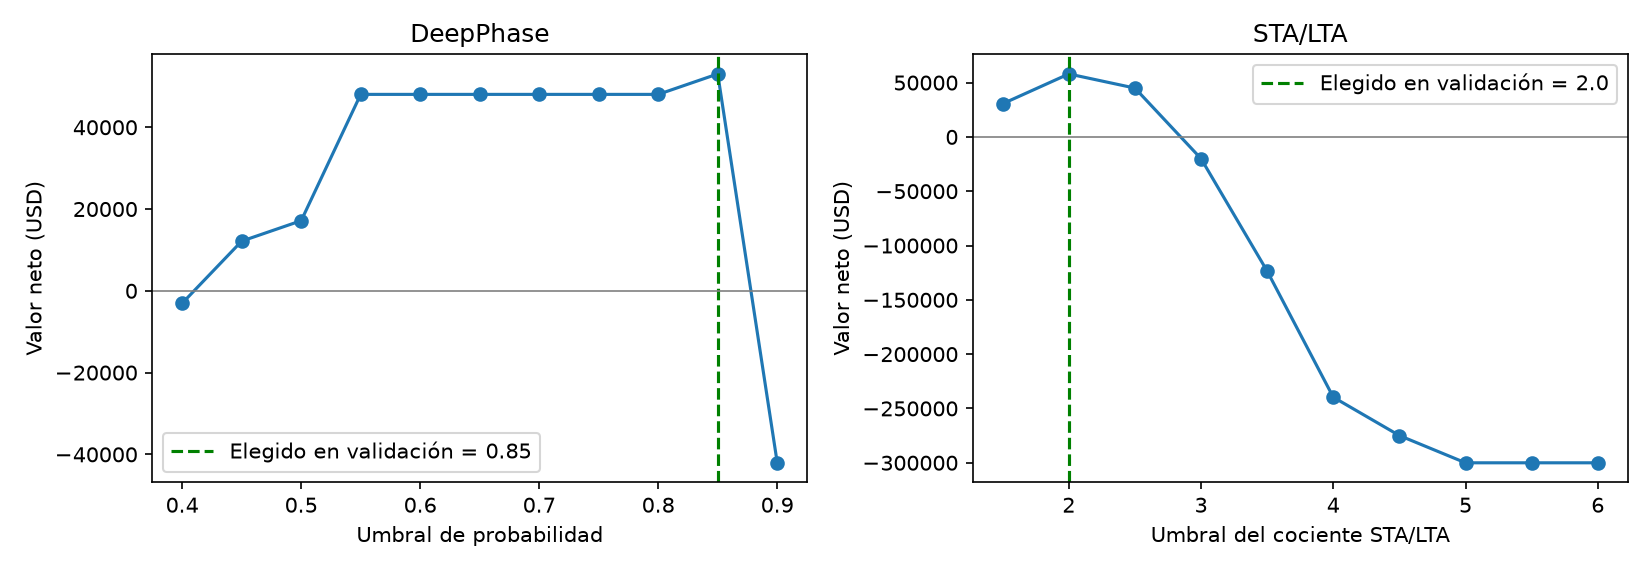
\includegraphics[width=\textwidth]{../results/value_curve.png}
\caption{Valor neto en el conjunto de prueba al variar el umbral.}
\label{fig:valor}
\end{figure}

\subsection{Análisis de sensibilidad}
Cada supuesto se varió $\pm$20~\% y $\pm$50~\% manteniendo los demás. La tabla
muestra el valor neto de DeepPhase en el umbral 0.85 (base: \$53,040).

\begin{table}[h]
\centering
\caption{Valor neto de DeepPhase en prueba al variar cada supuesto.}
\begin{tabular}{lrrrr}
\toprule
Supuesto & $-$50~\% & $-$20~\% & $+$20~\% & $+$50~\%\\
\midrule
$v_s$ (valor por segundo) & \$23,990 & \$41,420 & \$64,660 & \$82,090\\
$c_{fa}$ (falsa alarma) & \$55,540 & \$54,040 & \$52,040 & \$50,540\\
$c_{fn}$ (evento perdido) & \$53,040 & \$53,040 & \$53,040 & \$53,040\\
\bottomrule
\end{tabular}
\end{table}

El valor es sobre todo sensible a $v_s$, y su signo no cambia en ningún
escenario. $c_{fn}$ no afecta a DeepPhase en 0.85 porque en prueba no deja
eventos sin detectar, pero sí castiga a los umbrales más altos. El umbral
óptimo elegido en validación se mantiene en 0.85 en los 12 escenarios. La
diferencia con STA/LTA (que en su umbral óptimo de 2.0 no tiene falsos negativos
ni falsas alarmas) es negativa para DeepPhase en todos los escenarios, entre
--\$2,440 y --\$7,440: ningún supuesto económico razonable cambia el orden.

\section{Producto y experiencia de usuario}
Se ejecuta con \texttt{streamlit run src/app.py}. El operador selecciona si la
ventana contiene un evento, ajusta el umbral y pulsa ``Analizar ventana''. La
gráfica muestra la componente Z, las llegadas P/S verdaderas en la demo y las
detecciones. Se muestran simultáneamente DeepPhase, STA/LTA, probabilidad y
latencia. Ante una ventana sin detección se evita afirmar que no existe un
sismo; se informa que el umbral no fue alcanzado. Ante evento no detectado se
advierte que el resultado no es suficiente para producción.

\section{Limitaciones, riesgos y ética}
\begin{itemize}[leftmargin=*]
\item Las señales sintéticas no representan toda la geología, instrumentación,
  ruido ni distribución de magnitudes de Guatemala. La métrica sintética no es
  evidencia de desempeño operacional.
\item La detección P no estima por sí sola magnitud, epicentro ni intensidad.
  La onda S puede llegar antes por geometría y distancia; ``anticipación'' debe
  calcularse con un modelo físico y una red de estaciones.
\item Un falso negativo puede retrasar una acción de seguridad; un falso positivo
  puede detener una operación costosa. Por eso se reporta el valor y no solo F1.
\item No se deben conectar salidas del prototipo a maquinaria, gas o alarmas
  públicas. Se requiere validación sismológica, redundancia, fail-safe,
  calibración por estación, observabilidad y certificación.
\item STEAD y FDSN/IRIS deben citarse y usarse conforme a sus licencias y
  condiciones. No se incluyen datos personales ni credenciales.
\end{itemize}

\section{Iteraciones y trabajo futuro}
La iteración I0 es STA/LTA; I1 agrega el extractor de características y MLP;
I2 incorpora tres componentes y selección por umbral; I3 será fine-tuning de una
red de picking con STEAD y validación regional. En la siguiente fase se deben
comparar CNN 1-D, PhaseNet y EQTransformer, medir curvas precisión--recall,
calibración, error por SNR y desempeño por estación, y consultar FDSN/IRIS para
eventos guatemaltecos. Finalmente se debe desplegar un servicio de streaming con
ventanas solapadas, confirmación multiestación y un simulador del paro de
maquinaria.

\section{Conclusión y reproducción}
AlertaP convierte la propuesta en un producto ejecutable de extremo a extremo:
señal $\rightarrow$ procesamiento $\rightarrow$ modelo $\rightarrow$ alerta
$\rightarrow$ valor. La comparación justa STA/LTA/DeepPhase con costos explícitos
muestra que, en datos sintéticos de alta señal/ruido, el baseline clásico basta;
el valor del deep learning debe demostrarse con datos reales (STEAD) o
condiciones de ruido más exigentes, que es el trabajo pendiente. El código está en:
\url{https://github.com/AngelEsquit/PRYF-DL}

\begin{lstlisting}
python3 -m venv .venv
.venv/bin/pip install -r requirements.txt
.venv/bin/pytest -q
.venv/bin/python src/evaluate.py
.venv/bin/streamlit run src/app.py
\end{lstlisting}
\end{document}
